\chapter{Analysing Concurrent Systems}\label{chap:analysing_concurrent_systems} % (fold)
\begin{note}[Testing]
    Activity looking for \textit{failures} revealing faults
    \begin{definition}{Fault}{fault}
        A manifestation of an error: an action that produces an incorrect result
    \end{definition}
    \begin{definition}{Failure}{failure}
        When a \hyperref[def:fault]{fault} is encountered, it may result in a failure:
        \begin{itemize}
            \item a failure is related to expected functionality;
            \item a failure may be caused by many \hyperref[def:fault]{faults};
            \item a \hyperref[def:fault]{fault} can cause many failures;
        \end{itemize}
    \end{definition}
\end{note}
\begin{note}[Verification]
    Checking if the system satisfies its specification: ``have we built the system right?''.
    It's aimed at verifying that a property holds \textbf{for all possible scenarios (traces)}.
\end{note}
\begin{note}[Validation]
    Checking if the system satisfies customer's expectation: ``have we built the right system?'' 
\end{note}
\begin{note}[Testing]
    \textbf{Testing} is aimed at verifying that a (correctness) \textbf{property} holds for some selected scenarios, revealing the presence of errors, not their abscence
\end{note}
\begin{quote}[Livess and Safety Tests]
    There are two kinds of tests:
    \begin{itemize}
        \item \textbf{tests of safety}:
            \begin{itemize}
                \item verify that a class or system behaviour conforms to its specification;
                \item usually taking the form of testing \textbf{invariants};
                \item typically using \textit{assertions};
            \end{itemize}
        \item \textbf{tests of liveness}:
            \begin{itemize}
                \item progress/non-progress tests;
                \item harder to set up;
            \end{itemize}
    \end{itemize}
    \begin{warning}[Limitations]
        \begin{itemize}
            \item typically checking only a subset of the scenarios;
            \item ``\textit{heisenbugs}'' phenomenon: test code can introduce timing or synchronisation artefacts that can mask bugs;
        \end{itemize}
    \end{warning}
\end{quote}
%
\section{Verification}\label{sec:an_verification} % (fold)
For verification there are two principal formal techniques:
\begin{itemize}
    \item \textbf{model checking}: where verification is done by generating one by one all the states of the systems and by checking the properties state by state (it can be automated by \textbf{model checkers tools});
    \item \textbf{inductive proofs of invariants}: invariant properties are proved by \textit{induction} over the states of the system (it can be automated by tools called \textbf{deductive tools};
\end{itemize}
\begin{note}
    Both techniques rely on some kind of \textit{formal language}/\textit{calculus} to specify correctness properties
\end{note}
%
\subsection{Model Checking}\label{sub:an_model_checking} % (fold)
\textbf{Model Checking} is the most important and used technique for automatically checking correctness properties of concurrent systems: invaluable conceptual and practical tool for software engineers.
Strategy based on \textit{exhaustively searching the entire state space} of a system and verify if certain properties are satisfied:
\begin{itemize}
    \item properties as \textbf{predicates} on a system state or states, expressed as a logical specification such as propositional temporal logic formula;
    \item if the system satisfies the property, the model checker generates a \textit{confirmation} response, otherwise it produces a \textbf{trace}: useful to identify bugs not only to prove \textbf{correctness};
\end{itemize}
\begin{cimage}
    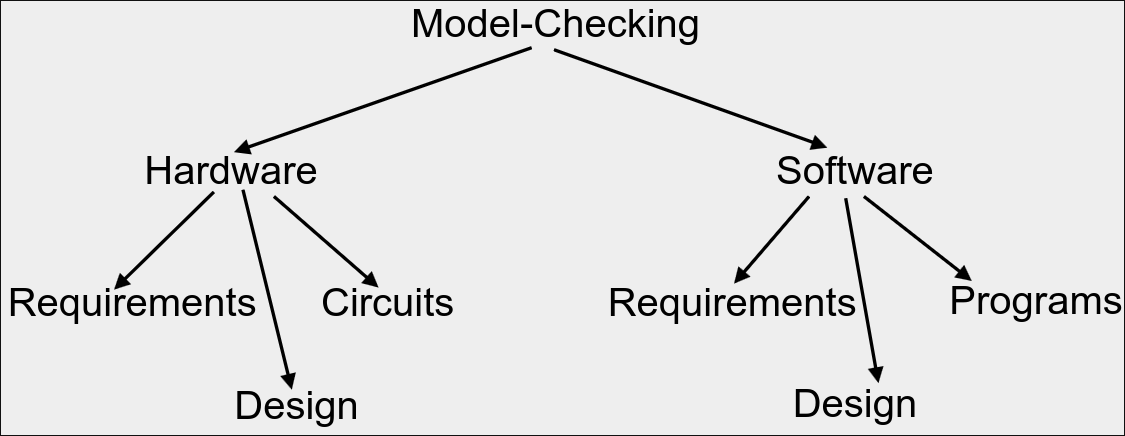
\includegraphics[width=.6\textwidth]{assets/20260928_093722.png}
    \caption{SW and HW model checking}\label{fig:20260928_093722}
\end{cimage}
\paragraph{State Space Explosion Problem}\label{par:an_state_space_explosion_probelm} % (fold)
The big problem of model checking technique is the \textbf{size of the state space}.
State-of-the-art techniques:
\begin{itemize}
    \item applying rules to reduce the number of states, using variables that can be modelled by a limited number of values;
    \item incremental construction of the whole graph:
        \begin{itemize}
            \item exploring only reachable state of an execution;
            \item checking the truth of a correctness specification as the incremental diagram is constructed, stopping the construction is a falsifying state is found;
        \end{itemize}
    \item \textit{symbolic} model checking, working with set of states;
\end{itemize}
% paragraph State Space Explosion Probelm (end)
%
\subsubsection{First Step: Specifying Properties}\label{sub:an_first_step_specifying_properties} % (fold)
A \textbf{property} is an attribute of a system that is true for every possible execution trace/scenario.
Properties of interest for concurrent programs fall into two categories: \textit{safety} and \textit{liveness}.
\begin{definition}{Safety Property}{safety-prop}
    A \textbf{safety property} asserts some condition that should be always verified:
    \begin{itemize}
        \item \textit{always} means in every possible state (of the \ac{lts});
        \item often specified using the negative version: some \textit{bad condition} that should never happen;
    \end{itemize}
\end{definition}
\begin{definition}{Liveness Property}{liveness-prop}
    A \textbf{liveness property} assets some condition that should eventually happen: \textit{eventually} means that in every execution/scenario the system must reach a state where the condition is true.
\end{definition}
% subsubsection First Step: Specifying Properties (end)
% subsection Model Checking (end)
%
\subsection{Properties in FSP}\label{sub:an_properties_in_fsp} % (fold)
Two main approaches:
\begin{itemize}
    \item ad hoc support: \textbf{property processes} or \textbf{progress properties};
    \item a more general support: \textbf{Fluents} and \textbf{Linear Temporal Logic};
\end{itemize}
%
\subsubsection{Safety Properties in FSP}\label{sub:an_safety_properties_in_fsp} % (fold)
\hyperref[def:safety-prop]{Safety properties} are specified in \ac{fsp} by \textbf{property processes}: simply \ac{fsp} processes prefixed by the keyword \texttt{property}.
They are composed with a target system to ensure that the specified property holds for that system.
\begin{example}{\texttt{POLITE} property example}{polit-prop}
    \begin{codeblock}{}
        property POLITE = (knock->enter->POLITE).
    \end{codeblock}
    \begin{cimage}
        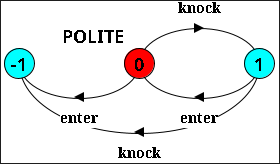
\includegraphics[width=.4\textwidth]{assets/20260928_095532.png}
    \end{cimage}
    \begin{note}
        Actions that are not part of the behaviour allowed by the safety property are transitions to the \texttt{ERROR} state
    \end{note}
\end{example}
\begin{critical}[Violations]
    A violation of the \texttt{POLITE} properties is an \texttt{enter} action before a \texttt{knock} action, or ``knocking'' twice
\end{critical}
\begin{definition}{}{}
    A \hyperref[def:safety-prop]{safety property $P$} defines a deterministic process that asserts that \textit{any trace} including actions in the alphabet of $P$, is accepted by $P$.
    Thus, if $P$ is  \hyperref[sub:md_parallel_composition_and_sequential_processes]{composed} with $S$, then traces of actions that are in the alphabet of $S$ and the alphabet of $P$, \textbf{must} also be valid traces of $P$, otherwise \texttt{ERROR} is reachable.
\end{definition}
So composing a property process with a set of processes does not affect their normal operation.
If a behaviour of $S$ can occur, violating the safety property, then a transition to the \texttt{ERROR} state results.
\begin{cimage}
    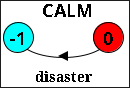
\includegraphics[width=.2\textwidth]{assets/20260928_101345.png}
\end{cimage}
\begin{note}
    Using alphabet extension to specify errors/condition that should never happen
\end{note}
% subsubsection Safety Properties in FSP (end)
%
\subsubsection{Liveness and Progress Properties}\label{sub:an_liveness_and_progress_properties} % (fold)
A \hyperref[def:liveness-prop]{liveness property} asserts something good eventually happens.
A completely general treatment of liveness is rather involved and requires the use of a temporal logic to specify the required liveness properties.
\emptyln{}
The \textbf{progress property} is a specific important case of liveness: it asserts that \textit{whatever state a system is in}, it is always the case that a specified action will eventually be executed.
\emptyln{}
Progress is the opposite of \textbf{starvation}, that is: the situation in which action is never executed, and the process is blocked.
\begin{note}
    Progress properties are simple to specify and are sufficiently powerful to capture a wide range of liveness problems in concurrent programs
\end{note}
% subsubsection Liveness and Progress Properties (end)
%
\subsubsection{Progress Property in FSP}\label{sub:an_progress_property_in_fsp} % (fold)
The definition of a progress property in \ac{fsp}:
\begin{codeblock}{}
    progress P = {a1,a2..an}
\end{codeblock}
The property asserts that in an \textbf{infinite} execution of a target system, at least one of the actions \texttt{a1,a2..an} will be executed \textbf{infinitely often}: in other words, a progress property asserts that at any stage of execution one of the actions in the progress set will eventually occur.
\begin{example}{Progress and the \texttt{COIN} system}{}
    \begin{codeblock}{}
    COIN = (toss->heads->COIN | toss->tails->COIN).
    \end{codeblock}
    The liveness requirement for coin tossing can now be expressed as:
    \begin{codeblock}{}
    progress HEADS = {heads}
    progress TAILS = {tails}
    \end{codeblock}
\end{example}
\begin{example}{Variation of the \texttt{COIN} system violating the progress property}{}
    \begin{codeblock}{}
    TWOCOIN = (pick -> COIN | pick -> TRICK).
    COIN = (toss->heads->COIN | toss->tails->COIN).
    TRICK = (toss->heads->TRICK).

    progress HEADS = {heads}
    progress TAILS = {tails}
    \end{codeblock}
    \begin{cimage}
        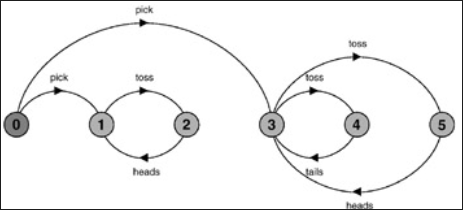
\includegraphics[width=.6\textwidth]{assets/20260928_102758.png}
    \end{cimage}
    Progress analysis of the \texttt{TWOCOIN} system against the progress properties \texttt{HEADS} and \texttt{TAILS} detects the violation of the progress \texttt{TAILS}.
    Instead, the progress property \texttt{HEADSorTAILS = \{heads, tails\}} would be satisfied
\end{example}
% subsubsection Progress Property in FSP (end)
% subsection Properties in FSP (end)
%
\subsection{Logical Description of Properties}\label{sub:an_logival_description_of_properties} % (fold)
\begin{definition}{Logical Description}{}
    A \textbf{Logical Description} is an expression composed out of propositions by logical operators such as and, or, not.
    \\
    A \textbf{proposition} is a statement that is either \red{true} or \red{false}.
    It can be formed from more primitive propositions by the logical operators and so the overall logical description is itself a proposition.
\end{definition}
\begin{quote}
    Proposition calculus is not enough
\end{quote}
In our models, we wish to specify propositions that are true for every possible execution of a program without explicit reference to a particular point in the execution of that program.
\\
A logic that permits us to do this is \textbf{\ac{ltl}}.
%
\subsubsection{Temporal Logic}\label{sub:an_temporal_logic} % (fold)
Processes and systems change their state over the time, and then also the interpretation of formulae about their state can change over the time.
\begin{definition}{Temporal Logic}{}
    The \textbf{temporal logic} is a formal logic obtained by adding temporal operators to propositional or predicate logic:
    \begin{itemize}
        \item \textbf{\acf{ltl}} to express properties that must be true (at a state) for every possible scenario (linear/discrete model of time);
        \item \textbf{Branching Temporal Logics} to express properties that must be true in some or all scenarios starting from a state (\textbf{\ac{ctl}});
    \end{itemize}
\end{definition}
% subsubsection Temporal Logic (end)
% subsection Logival Description of Properties (end)
%
\subsection{LTL: Temporal Operators}\label{sub:an_ltl_temporal_operators} % (fold)
\ac{ltl} is based on two basic temporal operators: \textit{always} and \textit{eventually}:
\begin{itemize}
    \item \textbf{box} or \textbf{always} temporal operator: $\cbox \textbf{p}$
        The formula $\cbox p$ is true in a state $s$ of a computation if and only if the formula $p$ is true in \textit{all states} following $s$:
        \[
            \cbox p = G\, p
        \]
        \begin{note}
            The \textit{always} operator can be used then to specify \hyperref[def:safety-prop]{safety properties}, because it specifies what must be always be true.
        \end{note}
    \item \textbf{diamond} or \textbf{eventually} temporal operator: $\dm \textbf{p}$
        The formula $\dm p$ is true in a state $s$ of a computation if and only if the formula $p$ is true in \textit{some} states following $s$:
        \[
            \dm p = F\, p
        \]
        \begin{note}
            The eventual operator is used to specify \hyperref[def:liveness-prop]{liveness properties}, because it specifies something that eventually be true. 
        \end{note}
\end{itemize}
\paragraph{Properties}\label{par:temp_properties} % (fold)
\begin{itemize}
    \item \textbf{Reflexivity}
        \begin{itemize}
            \item $\cbox p \to p$
            \item $p \to \dm p$
        \end{itemize}
    \item \textbf{Duality}
        \begin{itemize}
            \item $\neg \cbox p \to \dm\neg p$
            \item $\neg\dm p \to \cbox\neg p$
        \end{itemize}
    \item \textbf{Sequences of operators}
        \begin{itemize}
            \item $\dm\cbox p$
            \item $\cbox\dm p$
        \end{itemize}
\end{itemize}
% paragraph Properties (end)
%
\subsubsection{Deduction with Temporal Logic}\label{sub:an_deduction_with_temporal_logic} % (fold)
Temporal logic is a formal system of deductive logic with its own axioms and rules of inference: it can be used to \red{formalise} the semantics of concurrent programs and used to rigorously prove correctness properties of programs.
\begin{example}{}{}
    \begin{itemize}
        \item $(\dm\cbox p \land \dm\cbox q) \to \dm\cbox (p\land q)$ is \textbf{true}
        \item $(\cbox\dm p \land \cbox\dm q) \to \cbox\dm (p\land q)$ is \textbf{false}
    \end{itemize}
\end{example}
A proposition in \ac{ltl} logic describes a set of infinite sequences for which the proposition is true.
A system execution is essentially a sequence of states and so a system specification satisfies a linear temporal logic proposition \textit{if all its executions belong to the set described by the formula}.
% subsubsection Deduction with Temporal Logic (end)
%
\subsubsection{Fluents}\label{sub:an_fluents} % (fold)
\begin{definition}{Fluents}{}
    A \textbf{fluent} is a logical condition that \textbf{changes over time}.
    They are used in different contexts and can be expressed in different ways depending on the context.
    \emptyln{}
    In \ac{fsp} a fluent is defined as:
    \begin{codeblock}{}
    fluent FL = <{s1,...sn},{e1..en}> initially B
    \end{codeblock}
    It represents a fluent $FL$ that is initially true if the expression $B$ is true and initially false if the expression $B$ is false
    \\
    $FL$ becomes \red{true} when \textbf{any of the initiating actions \texttt{\{s1,...sn\}} occur} and \red{false} when \textbf{any of the terminating actions \texttt{\{e1..en\}} occur}.
    \begin{note}
        If the term \texttt{initially B} is omitted then $FL$ is initially false
        \begin{critical}
            The same action may not be used as both an initiating and terminating action
        \end{critical}
    \end{note}
\end{definition}
\begin{quote}
    Fluents holds at a time instant if and only if it holds initially or some initiating action has occurred, and, in both cases, no terminating action has yet occurred
\end{quote}
\begin{example}{Fluent Example}{}
    The following fragment defines a fluent \texttt{LIGHT} which becomes true when the action \texttt{on} occurs and false when the action \texttt{off} or \texttt{power\_cut} occurs.
    \begin{codeblock}{}
    const False = 0
    const True = 1
    fluent LIGHT = <{on}, {off, power_cut}> initially False
    \end{codeblock}
    This captures the state of a light so that when the light is on, the fluent \texttt{LIGHT} is true and when the light is off, the fluent is false.
    \\
    We can define indexed families of fluents in the same way that we define \hyperref[sub:md_indexed_processes_and_actions]{indexed families of processes}:
    \begin{codeblock}{}
    fluent LIGHT[i:1..2] = <{on[i]}, {off[i], power_cut}>
    \end{codeblock}
    This is equivalent to defining two fluents:
    \begin{codeblock}{}
    fluent LIGHT_1 = <{on[1]}, {off[1], power_cut}>
    fluent LIGHT_2 = <{on[2]}, {off[2], power_cut}>
    \end{codeblock}
\end{example}
% subsubsection Fluents (end)
%
\subsubsection{Action Fluents}\label{sub:an_action_fluents} % (fold)
\begin{definition}{Action Fluents}{}
    \textbf{Action fluents} are fluents defined directly for actions representing the condition: ``the action has just been executed''; they are represented directly by the name of the action.
    \emptyln{}
    They are defined by a set of initiating actions and a set of terminating actions.
    Consequently, given the alphabet $\al$ of a system, \textbf{we can define a fluent for each action $a$ in that alphabet} such that the initiating set of actions for the fluent $a$ is \texttt{\{a\}} and the terminating set of actions is \texttt{$\al\,\cup$ \{$\tau$\} - \{a\}.}
    \begin{note}
        That is the fluent for an action becomes true immediately that action occurs and false immediately the next action occurs: the next action may be the silent action $\tau$.
    \end{note}
\end{definition}
\begin{warning}
    We can also use a set of actions in a fluent expression: the logical value of this is disjunction (or) of each of the actions in the set
\end{warning}
% subsubsection Action Fluents (end)
%
\subsubsection{Fluent Expressions}\label{sub:an_fluent_expressions} % (fold)
We can combine fluents with the normal logical operators.
For instance:
\begin{itemize}
    \item if we wished to characterise the state in which two lights are on, this would be the expression \texttt{LIGHT[1] \&\& LIGHT[2]}
    \item the state in which either light is on would be \texttt{LIGHT[1] || LIGHT[2]}
\end{itemize}
Fluent expressions can be formed using the following logical operators:
\begin{itemize}
    \item \texttt{\&\&} conjunction (and) \texttt{||} disjunction (or);
    \item \texttt{!} negation (not);
    \item \texttt{->} implication \texttt{((A->B) $\equiv$ (!A||B))};
    \item \texttt{<->} equivalence \texttt{((A<->B) $\equiv$(A->B)\&\&(B->A))};
\end{itemize}
\begin{note}
    Expressions can flexibly combine action fluents and explicitly defined fluents, for instance: \texttt{getKey \&\& LIGHT[i]}: it is true when the \texttt{getKey} action occurs and the \texttt{LIGHT} fluent is true
\end{note}
\begin{example}{}{}
    Given the fluents:
    \begin{codeblock}{}
    fluent POWER = <power_on, power_off>
    fluent LIGHT = <on, off>
    \end{codeblock}
    the expression:
    \begin{codeblock}{}
    LIGHT->POWER
    \end{codeblock}
    states our expectation that, for the light to be on, the power must also be on
    \begin{warning}
        We do not expect that if the power is on the light need necessarily be on as well
    \end{warning}
\end{example}
% subsubsection Fluent Expressions (end)
%
\subsubsection{\texttt{forall} And \texttt{exists} Expressions}\label{sub:an_forall_and_exists_expressions} % (fold)
If we wish to express the proposition that all lights are on, we can use the expression: \texttt{forall[i:1..2] LIGHT[i]}
\begin{note}
    This is exactly the same as \texttt{LIGHT[1] \&\& LIGHT[2]}
\end{note}
Similarly, if we wish to express the proposition that at least one light is on, we can state: \texttt{exists[i:1..2] LIGHT[i]}
\begin{note}
    This is exactly the same as \texttt{LIGHT[1] || LIGHTS[2]}
\end{note}
% subsubsection \texttt{forall} and \texttt{exists} Expressions (end)
%
\subsubsection{Fluents with Temporal Operators}\label{sub:an_fluents_with_temporal_operators} % (fold)
Fluents let us express properties about the abstract state of a system at a particular point in time: this state depends on the trace of actions that have occurred up to that point in time.
\emptyln{}
To express propositions with respect to an execution of a model, we will use \ac{ltl}, introducing the two operators seen before: $\cbox F$ and $\dm F$
\begin{itemize}
    \item The linear temporal logic formula $\cbox F$ --- \textbf{always F} --- is true if and only if the formula $F$ is true at the current instant and at all instants in the future (used to express \hyperref[def:safety-prop]{safety properties};
    \item The linear temporal logic formula $\dm F$ --- \textbf{eventually F} --- is true if and only if the formula $F$ is true at the current instant or at some instant in the future (used to express \hyperref[def:liveness-prop]{liveness properties};
\end{itemize}
% subsubsection Fluents with Temporal Operators (end)
%
\subsubsection{Critical Sections}\label{sub:an_critical_sections} % (fold)
\begin{definition}{Critical Section}{}
    A \textbf{critical section} is a sequence of actions that a process has which satisfies the \textit{mutual exclusion} property so that is only one process at a time should be inside its critical section.
\end{definition}
\begin{example}{Two \texttt{USER} processes in critical section}{crit-sec-problem}
    \begin{codeblock}{}
    USER = (ncs->enterCS->cs->exitCS->USER).
    ||USERS = (a:USER || b:USER).
    \end{codeblock}
    In this case the \hyperref[sub:an_properties_in_fsp]{property} is violated: there are scenarios in which both the users are inside the critical section, executing \texttt{cs}.
    \emptyln{}
    The abstract states of interest here are when each \texttt{USER} processes enters its critical section.
    We express these states with \hyperref[sub:an_fluents]{fluents}:
    \begin{codeblock}{}
    fluent USER_A_IN_CS = <a.enter, a.exit>
    fluent USER_B_IN_CS = <b.enter, b.exit>
    \end{codeblock}
    The mutual exclusion property can be expressed by the \ac{ltl} formula:
    \[
        \text{MUTEX} = \cbox!\pt{\text{USER\_A\_IN\_CS \&\& USER\_B\_IN\_CS}}
    \]
    \begin{note}
        That is: the condition \texttt{!(USER\_A\_IN\_CS \&\& USER\_B\_IN\_CS)} must be true in every state
    \end{note}
    In \ac{fsp} the property can be specified using assert:
    \begin{codeblock}{}
    assert MUTEX = []!(USER_A_IN_CS && USER_B_IN_CS)
    \end{codeblock}
\end{example}
\paragraph{Solving the Problem with a Lock}\label{par:an_solving_the_problem_with_a_lock} % (fold)
The \hyperref[ex:crit-sec-problem]{critical section problem} can be solved by introducing a shared \texttt{LOCK} process, functioning as a lock that each user process has to acquire to before entering in \texttt{CS} and releases before exiting:
\begin{codeblock}{}
    USER = (ncs -> acquire->enterCS -> cs -> exitCS -> release->USER).
    LOCK = (acquire -> release -> LOCK).
    ||USERS =
    (a:USER || b:USER || {a,b}::LOCK).
    fluent USER_A_IN_CS = < a.enterCS, a.exitCS >
    fluent USER_B_IN_CS = < b.enterCS, b.exitCS >
    assert MUTEX = []!(USER_A_IN_CS && USER_B_IN_CS)
\end{codeblock}
In this case the property is verified.
% paragraph Solving the Problem with a Lock (end)
% subsubsection Critical Sections (end)
% subsection LTL: Temporal Operators (end)
%
\subsection{Liveness Properties using Eventually Operator}\label{sub:an_liveness_properties_using_eventually_operator} % (fold)
\hyperref[def:liveness-prop]{Liveness properties} specify conditions that eventually must become true, in every possible scenario, typically used to express progress properties.
\begin{note}[No Starvation]
    Critical section problem case study: \textit{if a user requests to enter in its \texttt{CS}, then eventually he/she will enter}
\end{note}
We can express this property using the temporal formula:
\begin{codeblock}{}
    assert NO_STARV =[](a.acquire -> <> a.enterCS)
\end{codeblock}
% subsection Liveness Properties using Eventually Operator (end)
%
\subsection{Further Operators of FLTL}\label{sub:an_further_operators_of_fltl} % (fold)
Beside the \textbf{always} operator $\cbox$ and eventually operator $<>$, some other \hyperref[sub:an_ltl_temporal_operators]{temporal operators} can be used in expressing properties:
\begin{itemize}
    \item \textbf{until} $U$
    \item \textbf{weak until} $W$
\end{itemize}
%
\subsubsection{Until Operator}\label{sub:an_until_operator} % (fold)
\begin{definition}{Until Operator}{}
    The linear temporal logic formula \texttt{p U q} is true if and only if $q$ is true at the current instant or if $q$ is true at some instant in the future and $p$ is true until that instant.
\end{definition}
\begin{example}{}{}
    Let's suppose we wish to assert the \hyperref[ex:polit-prop]{politeness property} that we should not enter a room before knocking.
    We can assert:
    \begin{codeblock}{}
    assert POLITE = (!enter U knock)
    \end{codeblock}
    This asserts both the safety property that we cannot have an enter action before a knock action, and also that a knock action should eventually happen.
\end{example}
%
\paragraph{\texttt{MUTEX} Using \texttt{UNTIL}}\label{par:an_texttt_mutex_using_texttt_until} % (fold)
Given the \hyperref[sub:an_until_operator]{until operator}, we can state the mutual exclusion property seen for the critical section problem using only \hyperref[sub:an_action_fluents]{action fluents}:
\begin{codeblock}{}
    assert MUTEX_U =
        []((a.enterCS -> (!b.enterCS U a.exitCS)) &&
        (b.enterCS -> (!a.enterCS U b.exitCS)))
\end{codeblock}
This expresses the required mutual exclusion safety property and, in addition, the \hyperref[def:liveness-prop]{liveness property} that if a process enters the critical section it should eventually exit.
% paragraph \texttt{MUTEX} using \texttt{UNTIL} (end)
%
% subsubsection Until Operator (end)
%
\subsubsection{Weak Until}\label{sub:an_weak_until} % (fold)
\begin{definition}{Weak Until}{}
    The linear temporal logic formula $p W q$ is true if and only if either $p$ is true indefinitely or if $p U q$.
    The difference with the previous definition of until is that this definition does not insist that $q$ eventually happens. The formula also holds if $p$ is true indefinitely.
\end{definition}
\begin{example}{Using weak until for the \hyperref[ex:polit-prop]{\texttt{POLITE} property}}{}
    \begin{codeblock}{}
    assert POLITE_W = (!enter W knock)
    \end{codeblock}
    \begin{warning}
        The property becomes a \hyperref[def:safety-prop]{safety property} since it no longer requires that knock eventually happens
    \end{warning}
\end{example}
% subsubsection Weak Until (end)
%
\subsubsection{Equivalences}\label{sub:an_equivalences} % (fold)
We can define the temporal operator always $\cbox$, eventually $\dm$ and weak until $W$ in terms of the until $U$ operator as follows:
\begin{itemize}
    \item[] \texttt{<> p $\equiv$ True U p}
    \item[] \texttt{[] p $\equiv$ !<>!p}
    \item[] \texttt{p W q $\equiv$ []p || (p U q)}
\end{itemize}
% subsubsection Equivalences (end)
%
\subsubsection{Rigid Expressions}\label{sub:an_rigid_expressions} % (fold)
Actually FLTL does not have the explicit constants True and False, instead it permits boolean expressions of constants and parameters.
These expressions are termed \textit{rigid}, since, unlike \hyperref[def:fault]{faults} propositions, they do not change truth value with the passage of time as measured by the occurrence of events.
\\
Thus, we can define:
\begin{codeblock}{}
    assert True = rigid(1)
    assert False = rigid(0)
\end{codeblock}
% subsubsection Rigid Expressions (end)
% subsection Further Operators of FLTL (end)
% section Verification (end)
% chapter Analysing Concurrent Systems (end)
